\documentclass[11pt,a4paper]{article}

% Enhanced packages for better typography and layout
\usepackage[left=0.75in, right=0.75in, top=0.75in, bottom=0.75in]{geometry}
\usepackage{hyperref}
\usepackage{enumitem}
\usepackage[usenames,dvipsnames]{xcolor}
\usepackage{fontspec}
\usepackage{setspace}
\usepackage[explicit]{titlesec}
\usepackage{multicol}
\usepackage{fontawesome5}
\usepackage{graphicx} % For including images

% Modern font selection
\setmainfont{Helvetica Neue}[
    UprightFont = *-Light,
    BoldFont = *-Bold,
]
\setsansfont{Arial}

% Custom colors
\definecolor{primarycolor}{RGB}{0, 79, 159}
\definecolor{secondarycolor}{RGB}{100, 100, 100}
\definecolor{linkcolor}{RGB}{0, 112, 201}
\definecolor{headerbg}{RGB}{240, 240, 240}

% Custom section styling
\titleformat{\section}
    {\LARGE\bfseries\color{primarycolor}\sffamily}
    {}{0em}
    {#1\hrule height 0.5pt \vspace{-1em}}

\titleformat{\subsection}
    {\bfseries\color{secondarycolor}\sffamily}
    {}{0em}{#1\vspace{-0.5em}}

% List styling
\setlist[itemize]{
    leftmargin=*,
    topsep=0.2em,
    itemsep=0.2em,
    parsep=0pt,
    label=\textbullet
}

% Hyperlink setup
\hypersetup{
    colorlinks=true,
    linkcolor=linkcolor,
    urlcolor=linkcolor,
    pdftitle={Evgeny Oleynik CV},
    pdfauthor={Evgeny Oleynik}
}

\begin{document}

% Header
\begin{center}
    \colorbox{headerbg}{\parbox{\textwidth}{
        \vspace{0.5em}
        \hspace{0.25em}
        \begin{minipage}[c]{0.2\textwidth}
            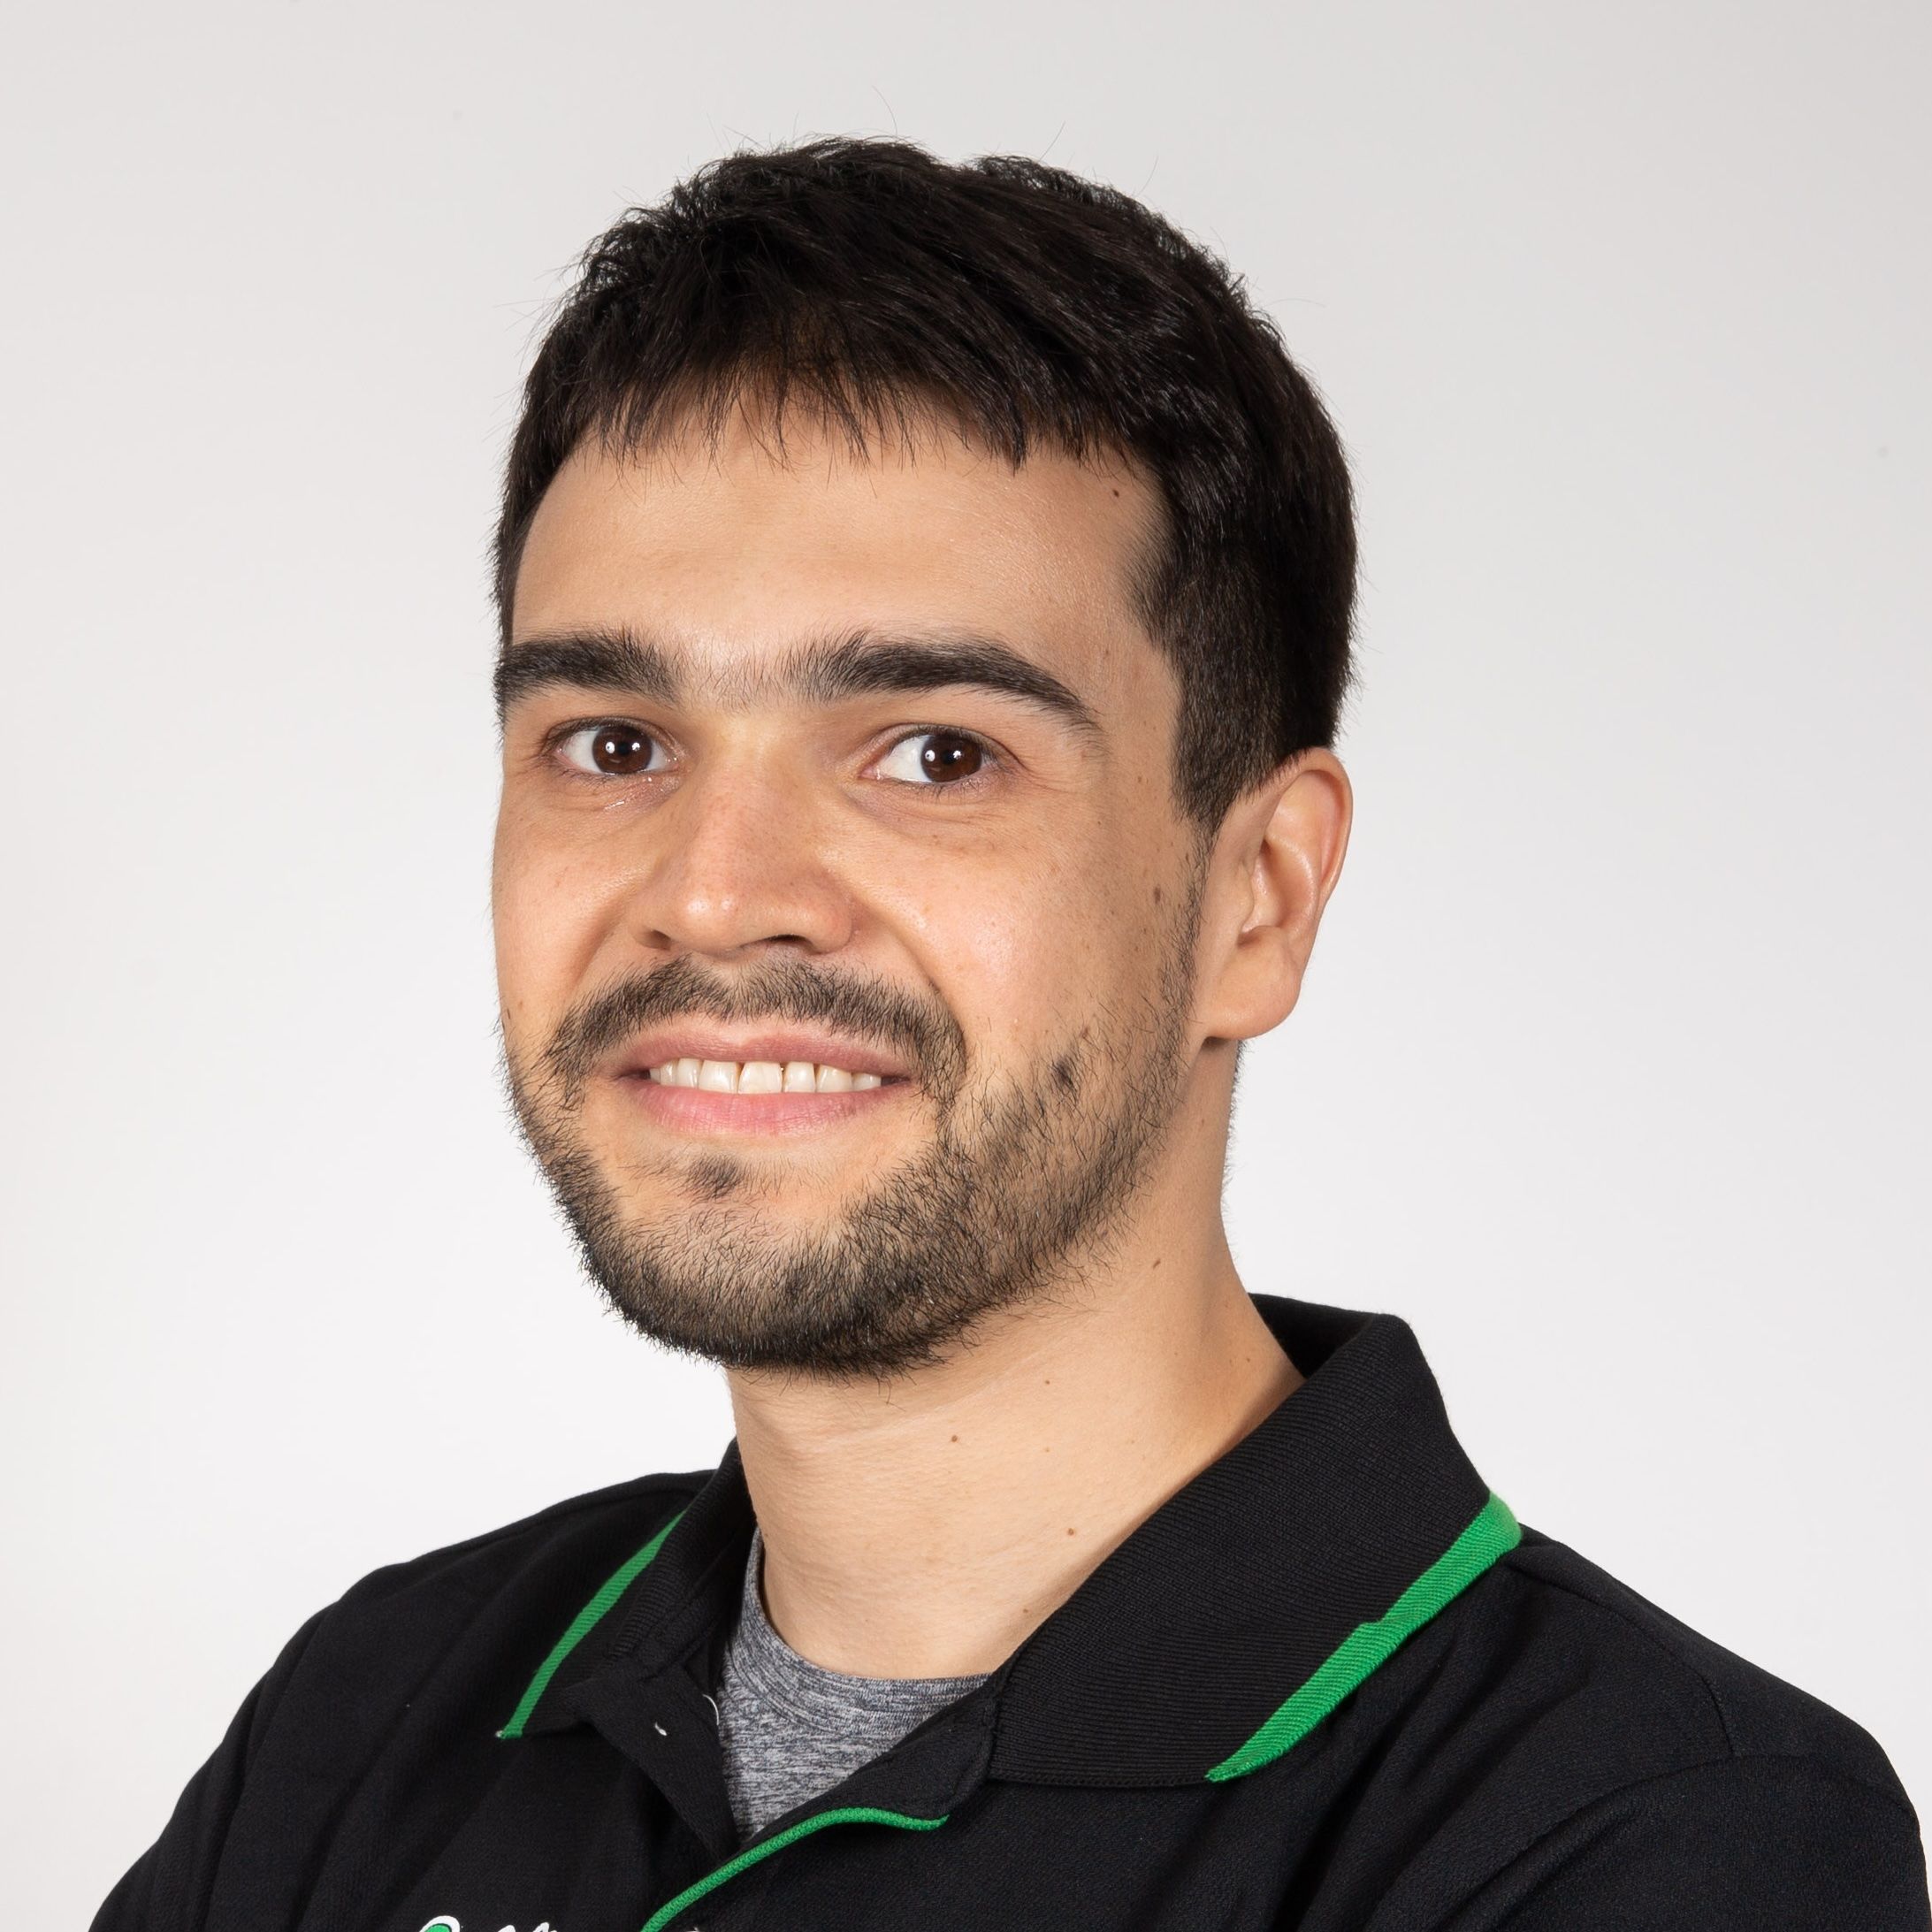
\includegraphics[width=\linewidth]{headshot.jpg} % Adjust the filename and path
        \end{minipage}\hspace{0.5em}\hfill
        \begin{minipage}[c]{0.75\textwidth}
            {\Huge\textbf{Evgeny Oleynik}} \\[0.3em]
            {\Large\color{secondarycolor} Co-Founder \& CTO, AirShelf AI | Agentic Commerce Infrastructure} \\[0.5em]
            {\color{secondarycolor}
            \faMapMarker \, Singapore \\[0.2em]
            \faEnvelope \, \href{mailto:evoleinik@gmail.com}{evoleinik@gmail.com} | \faPhone \, +65 8272 3349 \\[0.2em]
            \faLinkedin \, \href{http://linkedin.com/in/evoleinik}{linkedin.com/in/evoleinik} | \faGlobe \, \href{https://airshelf.ai}{airshelf.ai}}
        \end{minipage}
        \vspace{0.5em}
    }}
\end{center}

% Professional Summary
\section*{Professional Summary}
{\setstretch{1.2}
Technical founder building at the intersection of AI and commerce. Currently Co-Founder \& CTO of AirShelf AI (Antler-backed, Singapore), building infrastructure that makes brands discoverable and shoppable across AI agents. Previously Co-Founder \& CTO of 12Go, APAC's leading ground transportation OTA --- scaled to \textbf{30,000 bookings daily}, \textbf{45-person remote team}, and \textbf{\$500K daily GMV} over a decade. First paid enterprise pilot (Toshiba, \$20K) signed within 4 months of founding AirShelf.}

% Notable Achievements
\section*{Notable Achievements}
\begin{itemize}
    \item \textbf{Founded AirShelf AI} --- agentic commerce infrastructure making brands discoverable across AI agents. Antler-backed. First enterprise pilot (Toshiba, \$20K) signed within 4 months. Active pipeline includes Domino's Indonesia, Harvey Norman, HP, Dyson.
    \item \textbf{Scaled 12Go} from startup to APAC's leading ground transportation OTA, managing \textbf{45+ remote team members} across 12 departments and delivering \textbf{\$500K GMV daily} with \textbf{99.95\% uptime}.
    \item \textbf{Navigated the COVID-19 crisis} by executing operational pivots and leading due diligence for a successful M\&A integration across \textbf{4 international markets}.
    \item \textbf{Co-founded GV}, one of Southeast Asia's pioneering holiday rental platforms, partnering with Airbnb during their Thailand expansion.
\end{itemize}

% Professional Experience
\section*{Professional Experience}

\subsection*{Co-Founder \& CTO \hfill Oct 2025--Present}
\textbf{AirShelf AI | Agentic Commerce Infrastructure (Singapore)}
\begin{itemize}
    \item Building infrastructure that sits between retailers and AI agents --- ingests product data, enriches it into structured ``Decision Packs'' (Golden Record), and serves it to ChatGPT, Gemini, Perplexity, and any AI agent.
    \item Designed and shipped the full platform solo: Next.js dashboard, edge proxy for AI crawlers, semantic search API across 177 stores / 9 APAC markets, ACP/UCP protocol integration, and a verification pipeline that detects AI hallucinations against ground truth.
    \item First paid pilot: Toshiba (\$20K, live). Active pipeline: Domino's Indonesia (LOI signed), Harvey Norman, HP (via Garage 2.0), Dyson, Leroy Merlin.
    \item Selected for HP Garage 2.0 (Cohort 2) --- 21-country APAC network. Airwallex design partner for agentic payments.
    \item Stack: \textbf{TypeScript, Next.js, PostgreSQL (Neon), Prisma, Vercel, Redis, Gemini/GPT APIs}.
\end{itemize}

\subsection*{Founder in Residence (SG19) \hfill Sep--Nov 2025}
\textbf{Antler | Early-Stage VC (Singapore)}
\begin{itemize}
    \item Selected for Antler Singapore Cohort 19. Formed AirShelf with co-founder Ashish Piplani during the programme. Graduated with pre-seed investment.
\end{itemize}

\subsection*{Co-Founder \& Chief Technical Officer \hfill 2014--2024}
\textbf{12Go.com | Ground Transportation OTA (Online Travel)}
\begin{itemize}
    \item Co-founded and scaled a platform handling \textbf{30,000 tickets sold daily}, \textbf{100+ searches per second}, with \textbf{search latency under 150 ms}, \textbf{99.95\% uptime}, and \textbf{global coverage}.
    \item Unified a multicultural team spanning \textbf{Eastern Europe, Southeast Asia, Middle East}, managing \textbf{45 remote team members} across \textbf{12 departments}.
    \item Transitioned the company from a startup environment to corporate governance, integrating quarterly milestone planning and QBR reporting.
\end{itemize}

\subsubsection*{Leadership and Team Building}
\begin{itemize}
    \item Cultivated an \textbf{end-to-end ownership culture}, empowering teams to solve problems autonomously.
    \item Nurtured a \textbf{collaborative environment}, fostering respectful and productive discussions.
    \item Established KPIs for engineering teams, driving a \textbf{performance-driven culture}.
    \item Implemented \textbf{agile workflows}, delivering fortnightly and on-demand releases via CI/CD pipelines.
    \item Introduced \textbf{data-driven decision-making} using Jira Product Discovery (ICE prioritization) and A/B testing frameworks.
\end{itemize}

\subsubsection*{System Architecture and Development}
\begin{itemize}
    \item \textbf{Backend}: Led teams to build a scalable \textbf{search API} with latency under 150 ms, sharded caches, and a flexible pricing engine. Oversaw integration of \textbf{150+ supplier systems}.
    \item \textbf{Frontend}: Guided development of a modern web app using \textbf{Node.js, Vue.js, Nuxt} and a mobile app contributing \textbf{30\% of bookings} within its first year.
    \item \textbf{Infrastructure/DevOps}: Managed AWS infrastructure (\textbf{EC2, ELB, RDS, S3, CloudFront}) with tools like \textbf{Grafana}, \textbf{Datadog}, \textbf{Bugsnag}, and \textbf{Clickhouse}.
\end{itemize}

\subsubsection*{Strategic Contributions}
\begin{itemize}
    \item Partnered closely with the product team to deliver features on time and with high-quality code.
    \item Planned annual budgets for infrastructure, third-party tools, and hiring, aligning resources with business growth objectives.
    \item Navigated the COVID-19 crisis, leading due diligence for a successful M\&A with an Israeli group, integrating operations across \textbf{Israel, Croatia, Argentina, and Brazil}.
\end{itemize}

\subsection*{Co-Founder \& Chief Technical Officer \hfill 2011--2012}
\textbf{GV | Holiday Rentals Platform (Online Travel/PropTech)}
\begin{itemize}
    \item Co-founded one of Southeast Asia's first holiday rental platforms, partnering with Airbnb during their Thailand expansion.
    \item Engineered scalable backend systems using \textbf{PHP}, \textbf{MySQL}, and \textbf{Go}, supporting \textbf{thousands of property listings}.
    \item Expanded the business beyond Russian-speaking clients, achieving significant growth in Southeast Asia.
\end{itemize}

% Skills
\section*{Skills \& Expertise}
\begin{itemize}
    \item \textbf{AI \& LLM Integration}: Building production systems on top of OpenAI, Gemini, and Perplexity APIs. Semantic search, structured data extraction, hallucination detection, agent commerce protocols (ACP, UCP, MCP).
    \item \textbf{Full-Stack}: TypeScript, Next.js, React, Node.js, PostgreSQL, Prisma, Redis, Vercel. Previously PHP/Symfony, Vue.js, MySQL, Go.
    \item \textbf{System Architecture}: Designing low-latency, high-availability systems. Edge proxies, API design, caching, real-time pipelines.
    \item \textbf{Cloud \& Infrastructure}: AWS (EC2, RDS, S3, CloudFront), Vercel, Neon (serverless Postgres), Docker, K3s. Monitoring: Grafana, Datadog, Axiom.
    \item \textbf{Leadership}: Built and managed 45-person remote team across 12 departments. Hiring, mentoring, retention. Agile, CI/CD, data-driven prioritization.
    \item \textbf{Founder Skills}: Fundraising (Antler pre-seed), enterprise sales, pilot delivery, investor relations, M\&A due diligence.
\end{itemize}

% Education
\section*{Education}
\textbf{Specialist degree in Applied Mathematics} \\
Moscow Aviation Institute (National Research University) \hfill 2005--2010

% Additional Information
\section*{Additional Information}
\textbf{Languages:} Fluent in English and Russian (native), Thai (conversational) \\
\textbf{Location:} Singapore (previously Bangkok, 10+ years)

\end{document}
